\chapter{Automatický přepis}
\label{kap:asr}

% - množina hlásek
% - vektorový formát
% - HMM X CNN
% - HTK X Kaldi X sphinx X Bourlard X TensorFlow
% - Monofóny X trifóny
% - mixtury
%   - individuální
%   - globální
%   - na monofónech vs. trifónech



Koncept celého projektu se zakládá na~přítomnosti počátečního přepisu a jeho
následném zdokonalování.
Je tedy nutné opatřit způsob, jak korpus strojově převést do textové podoby. Tím
se dostáváme do oblasti z~historických důvodů zvané \textit{automatické
rozpoznávání řeči}, anglicky \textit{automated speech recognition}, zkracované
jako \textit{ASR}, ačkoliv z povahy věci by přesnějším výrazem byl
\textit{automatický přepis}.

Automatický přepis lze chápat jako úlohu transformace signálu nebo jako
rozpoznávání vzorců v~datech. Algoritmus takových úloh je obvykle velice
složitý, neboť variabilita vstupních dat je značná a také zadání je inherentně
vágní: mnohdy je i pro člověka obtížné rozeznat, jakou hlásku nebo jaké slovo
určitý zvuk představuje.

Řešení problému, jak systému předat potřebnou znalost mapování vstupních dat na
kýžený výstup, se řeší kombinací dvou přístupů: přímým zakomponováním lidské
expertizy a strojovým učením z~dat. Pojem strojové učení vznikl už v~roce
1959\cite{samuel1959some} a obor se od té doby rozvíjí a získává na popularitě.
Už legenda strojového zpracování přirozeného jazyka kladenský rodák Bedřich
Jelínek, lépe známý pod svým poangličtěným jménem Frederick Jelinek, proslul
svým výrokem, že kdykoliv vyhodí lingvistu, zvýší se mu úspěšnost systému.

Ve strojovém učení pracujeme s~pojmy \textit{trénovací data} a \textit{testovací
data}. V~obou případech se jedná o správně spárovaná vstupní a výstupní data.
V~případě ASR tedy jde o páry záznamů mluveného slova a odpovídajících přepisů.
Trénovací data jsou ta, která má systém k~dispozici, aby z~nich odvodil znalost
potřebnou pro danou úlohu, tedy v~našem případě pro převod zvuku do textu.
Testovací data jsou potom ta, na nichž se vyhodnocuje úspěšnost systému.

Toto vychází z~předpokladu, že v~trénovacích datech je zobecnitelná informace,
která platí i o testovacích datech. Také se vychází z~předpokladu, že testovací
data jsou od trénovacích striktně oddělena, neboť jedině tak lze na základě
výsledku testování vyvozovat relevanci i pro další, neznámá data.

V~mém případě je úloha specifická tím, že se nesnažím vyvinout systém na
univerzální predikci neznámých dat: Jedná se mi o přepis daného korpusu, který
mám celý k dispozici. Karel Makoň je po smrti, takže dalších nahrávek se od něho
nenadějeme. Testovací sada oddělená od trénovací je však podstatná pro
vyhodnocení, ze kterého se dá soudit o výkonu na částech korpusu, pro který
chybí ruční přepis.

Výhoda strojového učení oproti ručním pravidlům je zřejmá: v~datech je informace
uložena objektivně, pravdivě. Oproti tomu v~ručně psaných pravidlech je zanesen
lidský faktor, který s~sebou nese předpojatost, omylnost a nepřesnost. Strojový
čas je navíc mnohdy dostupnější než lidský.

Nevýhodou strojového učení je, že je k~němu zapotřebí trénovacích dat, a to čím
více, tím lépe, aneb ,,there is no data like more data``\footnote{Robert Mercer,
1985}. Je
známo, že neuronová síť i hloubky 1 je s~dostatečným počtem neuronů schopna
modelovat jakoukoliv spojitou funkci s~omezeným definičním oborem (Csáji
2001)\cite{csaji2001approximation}. Kdybychom tedy měli neomezeně mnoho
kvalitních trénovacích dat a výpočetní kapacity, nebylo by důvodu aplikovat
lidskou expertizu.

Jelikož jsou však zdroje omezené, tyjí systémy typicky z~obou zdrojů: z~lidské
odbornosti a strojového učení, přičemž historicky s~dokonalejšími počítači a
větším množstvím dat v~systémech ubývá jednoho a přibývá druhého.

\section{Vybrané milníky v~rozpoznávání řeči}

Již v~roce 1952 vyvinuly Bell Laboratories analogové obvody, které dokázaly pro
konkrétního mluvčího rozpoznat vyslovené číslice v~telefonním
přenosu.\cite{davis1952automatic}
Systémy v~sedmdesátých letech porovnávaly vstupní zvukový záznam
s~množinou předloh a výstup určili podle nejpodobnější
varianty\cite{huang2014historical}.
Porovnávání se šablonami má zásadní nevýhodu v~tom, že totéž slovo, ba tatáž
hláska může být pokaždé vyslovena jinak rychle, jinými slovy v~řeči je velká
časová variabilita. Ještě v~osmdesátých letech se tato technika namnoze
používala a časová variabilita se kompenzovala roztažením či smrsknutím vzorků,
aby si délkou odpovídaly. Tato metoda se anglicky nazývá \textit{dynamic time
warp} a vznikla v~roce 1971\cite{sakoe1971chiba}, viz obrázek~\ref{fig:dtw}.
V~těchto přístupech pochází veškerá expertiza ze strany člověka.

\begin{figure}[htpb]
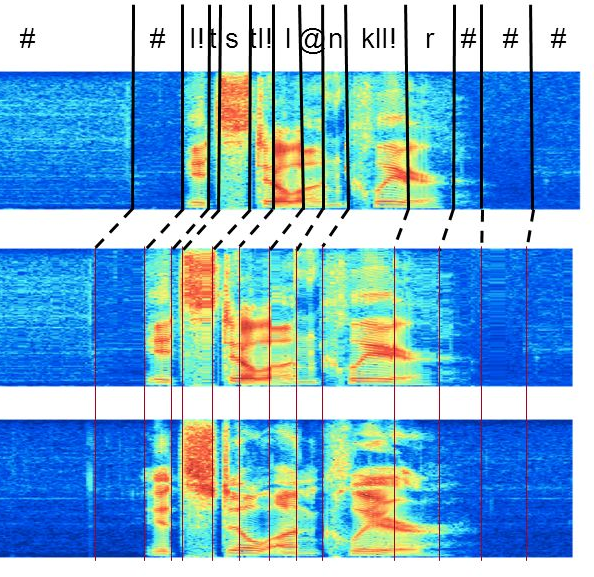
\includegraphics[scale=1]{rc/dtw.png}
\caption{
  Ilustrace rozpoznávání řeči pomocí šablon technikou dynamic time warp.
}
\label{fig:dtw}
\end{figure}

Velkým průlomem bylo použití skrytých markovovských modelů \textit{(Hidden
Markov Models, HMM)}. Vychází se z~představy, že mluvčí předává informaci
(posloupnost písmen, či slov) zakódovanou v~kanálu akustického vlnění, a naším
úkolem je původní informaci rozkódovat. Markovovské modely ve spojení
s~gaußovskými směsmi \textit{(Gaussian Mixture Models, GMM)} byly dominantní
technologií rozpoznávání řeči až do průlomu hlubokých neuronových sítí.

Hluboké učení přineslo zatím poslední skokový posun kupředu. Hluboké neuronové
sítě nejdříve vstupují jako součást schématu s~HMM, sloužíce pro odhad
aposteriorní pravděpodobnosti přepisu na základě akustických dat a nahrazujíce
složku GMM, čímž vznikají hybridní systémy DNN-HMM místo dosavadních GMM-HMM.
Posléze se objevují systémy realizované pomocí jedné neuronové sítě, která řeší
celou úlohu rozpoznávání.

\section{Kódování signálu}

Jedním z~nejdůležitějších stavebních prvků v~systémech rozpoznávání řeči je
předzpracování zvukové vlny do vhodnějšího formátu.

Zvukový signál je velmi prostý: je to spojitá funkce času do reálných čísel.
Má-li se zaznamenat digitálně, volí se technika vzorkování \textit{(sampling)},
kdy se z~průběhu funkce v~čase, jehož spojitost či diskrétnost je otázkou mimo
rámec této práce, vybere vzorek v~rozestupu definované periody, viz
obrázek~\ref{fig:sampling}. Čím větší
vzorkovací frekvence, tím 1) větší věrnost při reprodukci, 2) vyšší tónovou
frekvenci lze reprezentovat a 3) větší náročnost na uložení a zpracování.

\begin{figure}[htpb]
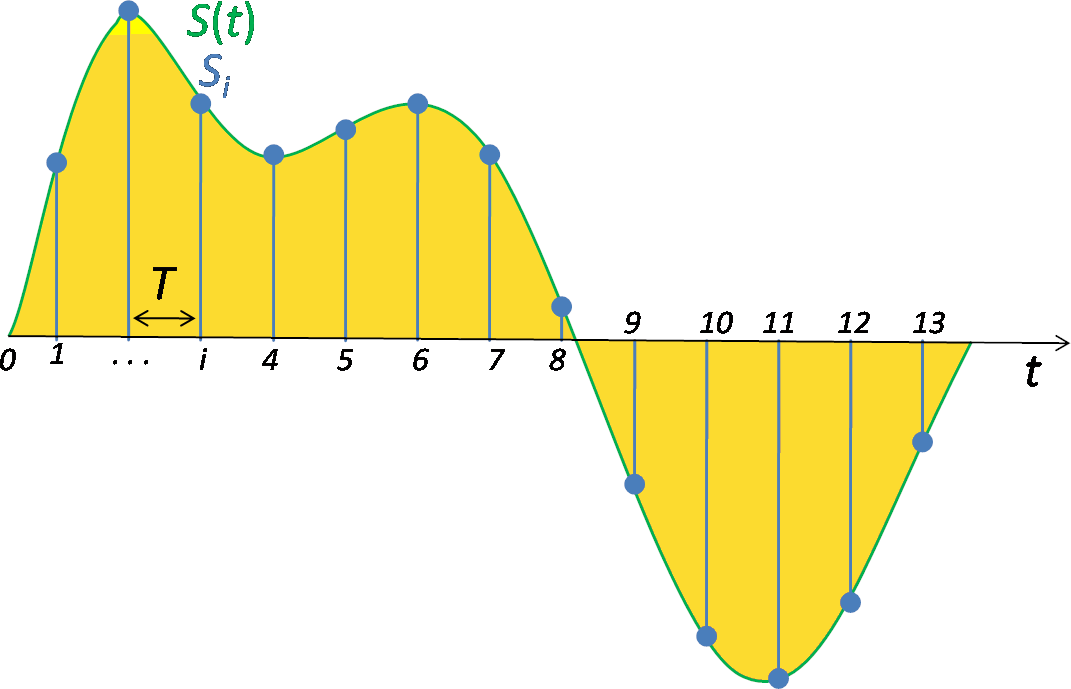
\includegraphics[scale=0.38]{rc/Signal_Sampling.png}
\caption{
    Vzorkování signálu. $t$ je čas, $S(t)$ je průběh signálu, $T$ je vzorkovací
    perioda, $S(i)$ je hodnota $i$-tého vzorku.
}
\label{fig:sampling}
\end{figure}

Vzorkovací frekvence se podle účelu záznamu pohybuje obvykle od 8~kHz pro
datově úsporný přenos hlasu do 96~kHz pro studiové zpracování hudby. Pro účely
rozpoznávání řeči se osvědčila vzorkovací frekvence 16~kHz jako minimum, ve
kterém je obsažena prakticky veškerá relevantní informace.

Jako vstupní data pro skryté markovovské modely nejsou prostá reálná
čísla\footnote{Pro počítačovou implementaci jsou reálná čísla díky svému
nekonečnému desetinnému rozvoji nereálná, pro se v~praxi pracuje s~tzv. čísly
s~plovoucí desetinnou čárkou (\textit{floating-point numbers}).} v~řádu tisíců
za sekundu praktická, pročež se signál nejdříve transformuje do jiné formy. Tato
část systému se zove \textit{front-end} a implementuje se nejčastěji pomocí
melfrekvenčních kepstrálních koeficientů \textit{(MFCC)} nebo řidčeji pomocí
perceptuální lineární predikce \textit{(PLP)}. Účelem není jen transformace do
praktičtějšího prostoru, ale též odstranění nerelevantní informace a normalizace
té relevantní.

Převod z~akustického vlnění do melfrekvenčních kepstrálních koeficientů\cite{mfcc1969}
transformuje proud jednoho reálného čísla šestnáctkrát za milisekundu do proudu
reálněčíselného vektoru stokrát za sekundu. Běžně každý vektor kóduje časové
okno o délce čtyřicetiny sekundy a okna jsou od sebe vzdálena setinu sekundy,
takže se překrývají, viz obrázek~\ref{fig:mfcc-windowing}. Na každém časovém
okně se provede diskrétní Fourierova transformace
\begin{equation}
X_k = \sum_{n=0}^{N-1} x_n \cdot e^{-\frac {i 2\pi}{N}kn}
\end{equation}
a rozdělí se do frekvenčních
oken podle škály
mel\cite{stevens1937scale} aplikováním trojúhelníkového filtru
\begin{equation}
Y_{t,m} = \sum_{k=1}^N W_m(k) |X_{t,k}|^2
\end{equation} kde $W_m$ je $m$-tý trojúhelníkový filtr a $k$ je index ve
výsledném vektoru DFT, viz
obrázek~\ref{fig:mfcc-mels}. Frekvenčních
oken bývá 12 a opět se překrývají. Frekvenční okna se s~rostoucí frekvencí
zvětšují tak, aby zůstávala konstantní v~jednotkách mel a aby tedy odpovídala
lidskému vnímání spektra. Hodnoty se logaritmují, opět aby byly
úměrnější lidskému vnímání hlasitosti. Jako třináctá hodnota se přidá buď
základní frekvence nebo častěji akustická energie.
\begin{equation}
E = \sum_{t=t_1}^{t_2}x^2_t
\end{equation}
Poté se provede inverzní
diskrétní Fourierova transformace. Od těchto hodnot se na základě kontextu přidá první a
druhá derivace,
\begin{equation}
d(t) = {{c(t+1) - c(t-1)}\over{2}}
\end{equation}
čímž získáváme devětatřicetirozměrný reálněčíselný vektor každou
setinu sekundy.

\begin{figure}[htpb]
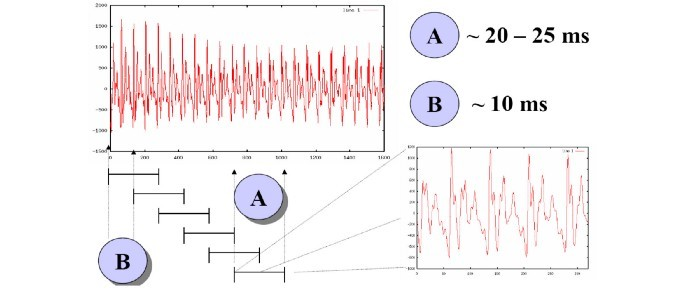
\includegraphics[scale=1]{rc/mfcc-windowing.jpg}
\caption{
    Schéma překrývajících se oken při převodu z~vlnového průběhu do
    melfrekvenčních kepstrálních koeficientů. $A$ je šířka okna, $B$ je rozestup
    mezi okny.
}
\label{fig:mfcc-windowing}
\end{figure}

\begin{figure}[htpb]
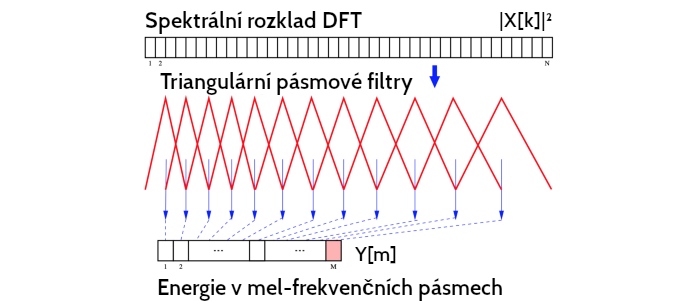
\includegraphics[scale=0.58]{rc/mfcc-mels.png}
\caption{
    Schéma aplikace filtrů do pásem podle stupnice mel.
}
\label{fig:mfcc-mels}
\end{figure}

\section{HMM}

V~této sekci stručně představím architekturu systémů rozpoznávání řeči založenou
na skrytých markovovských modelech, jak se běžně používala ještě na začátku
tohoto tisíciletí a této disertace.

Úlohu automatického rozpoznávání řeči můžeme formalizovat takto: Na základě vstupní
posloupnosti hodnot akustického vlnění $A$ hledáme takovou posloupnost slov
\textit{(words)} $W$, aby pravděpodobnost $P(W|A)$ byla co největší, tedy:

\begin{equation}
argmax_{\vec{W}} P(W|A)
\end{equation}

Pravděpodobnost $P(W|A)$ ovšem dlouho nebylo jak odhadnout, proto se využilo
Bayesova pravidla:

\begin{equation}
P(W|A) = {{P(A|W) P(W)}\over{P(A)}}.
\end{equation}.

Pravděpodobnost vstupních dat je ve vztahu k odhadovanému modelu konstantní a
kladná, proto se jmenovatel zanedbává. Zbývá tedy odhadnout $P(A|W)$ a $P(W)$.
Pro to první se vžilo název \textit{akustický model (AM)}, pro to druhé
\textit{jazykový model (language model, LM)}.

Akustický model je právě tím místem, které zastávají skryté markovovské modely.
Jedná se o generativní modelování, tedy pro účely řešení úlohy předpokládáme, že
vstupní akustická sekvence je generována markovovským procesem, viz
obrázek~\ref{fig:hmm}.

\begin{figure}[htpb]
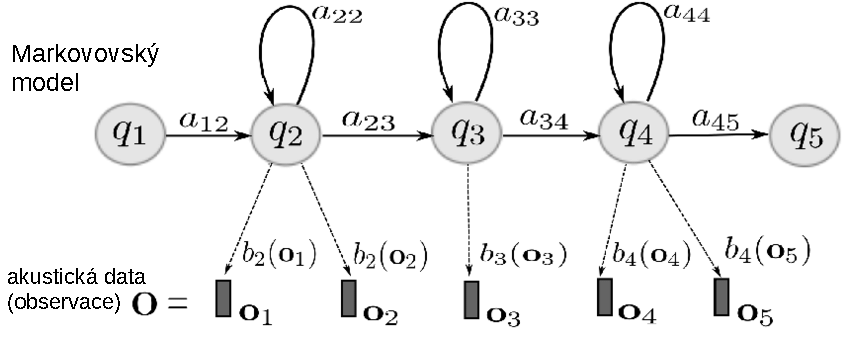
\includegraphics[scale=0.48]{rc/hmm.png}
\caption{
    Schéma použití markovovského řetězce jako generativního modelu
    v~rozpoznávání řeči.
}
\label{fig:hmm}
\end{figure}

Markovovský model realizuje akustický model jako sumu odhadnutých
pravděpodobností přechodů stavy automatu při pozorování dané vstupní
posloupnosti:

\begin{equation}
P(A|M) = \sum_X a_{x(0)x(1)} \prod_{t=1}^T b_{x(t)}(o_t)a_{x(t)x(t+1)}
\end{equation}

kde $x(0)$ je vstupní a $x(T + 1)$ výstupní stav modelu, $a_{xy}$ je přechodová
pravděpodobnost z~$x$ do $y$, $b_{x}$ je emisní pravděpodobnost symbolu $x$ a
$X$ je množina možných stavových posloupností.

Parametry, které HMM definují, jsou vymezení stavů v~prostoru vstupních dat a
přechodové pravděpodobnosti mezi stavy. Musí se tedy určit množina modelů a
prostor vstupních dat.

%\subsection{Prostor vstupních dat}


% over

V~prostoru vstupních dat, jak bylo řečeno, se musí vymezit stavy jednotlivých
markovovských modelů. Intuitivně si toto lze představit jako akustický popis
toho, jak vypadá spektrum, když se říká ta která hláska. Vymezení se provádí
pomocí pravděpodobnostní distribuce určené středem a variancí v~každé dimenzi.

Modelují se obvykle hlásky, ačkoliv v~úvahu přicházejí i slabiky nebo
v~některých jazycích s~kromobyčejně pravidelnou výslovností i přímo písmena.
V~obvyklém případě jednoho markovovského modelu pro každou hlásku se modely
definují jako pětistavové: vstupní stav, stav modelující počátek hlásky, stav
modelující prostředek hlásky, stav modelující konec hlásky a koncový stav. Krom
toho existuje model pro ticho, které zahrnujeme mezi hlásky, a model pro krátkou
pauzu, který je zvláštní tím, že může mít nulovou délku.

Přechodová matice se omezuje takto: Z~počátečního stavu se přejde vždy do
druhého. Z~vnitřních stavů se přejde vždy buď do následujícího nebo se setrvá.
Tak se nakonec vždy dá projít z~počátečního stavu do koncového.
Vzhledem k~tomu, že ticho modeluje i neřečové události a často odpovídá dlouhým
úsekům, povoluje se u něho, jakož i u krátké pauzy, přechod mezi druhým a
čtvrtým stavem v~obou směrech. Model pro krátkou pauzu sdílí stavy s~modelem
ticha, jen navíc umožňuje přechod z~počátečního stavu rovnou do koncového.

Až na ticho a krátkou pauzu má tedy každá přechodová matice třikrát dvě
pravděpodobnosti, které je potřeba natrénovat.
Jestliže pak rozeznáváme u češtiny čtyřicet jednu hlásku plus ticho plus
krátkou pauzu, bude tento jednoduchý akustický model mít
\begin{equation}
41 \times (6 + 2 \times 39) + 2 \times 39 + 8 + 9 = 3539
\end{equation}
volných parametrů.

Protože modelujeme hlásky a na výstupu očekáváme písmena, je potřeba adaptace na
obou stranách akustického modelu. Na straně vstupu jde o konverzi trénovacích
dat z~dvojic {\em promluva - ortografický přepis} do dvojic {\em promluva -
fonetický přepis}. Na straně výstupu jde o vytvoření výslovnostního slovníku,
kde každému slovu je přiřazena množina potenciálních výslovností. %S~tím také
%souvisí fakt, že ačkoliv jsme úlohu formulovali jako hledání ideální
%posloupnosti písmen, pracuje se obvykle se slovy jako elementárními jednotkami.
%To má několik důvodů: Za prvé je to právě kvůli výslovnostnímu slovníku: určit
%každému písmenu, jak se může vyslovovat, je nepraktické -- to se ozřejmí
%až na úrovni slov. Za druhé jazykové modelování je na slovech obvyklejší, což
%souvisí s~tím, že za třetí úspěšnost se měří na celých slovech.


Jazykový model je nástroj pro odhadování pravděpodobnosti konkrétního textu.
Praktický monopol zde mají tzv. n-gramové modely, kde se pravděpodobnost
odhaduje přes počty výskytů konkrétních slov, dvojic slov, až n-tic slov v~daném
korpusu. Až v~poslední době se objevují sofistikovanější přístupy s~využitím
rekurentních neuronových sítí.

Volné parametry akustického modelu se odhadují Baum-Welchovým iterativním
algoritmem\cite{welch2003hidden} taktéž na základě trénovacích dat. Oba základní stavební kameny:
akustický i jazykový model tedy svoji efektivitu získávají z~dat, takže značná
část expertizy systému pochází z~nich, nikoliv již z~lidské ruky.

Důležitým zdokonalením systému je rozšíření množiny markovovských modelů.
Jednotlivé realizace hlásek se od sebe tak odlišují, že modelovat např. všechny
výskyty hlásky ,,h`` jedním modelem je nedostačující. Zavádí se proto kontext:
Místo jednoho modelu pro danou hlásku máme model pro hlásku v~kombinaci
s~předchozí a následující hláskou. Je-li hlásek 42 (včetně ticha), pak nyní
bude modelů $42^3 = 74088$. 42 je příliš málo, 74088 je příliš mnoho. Navíc se
od sebe hlásky liší jen v~některých kontextech. Ještě navíc se jich většina
vůbec nevyskytne v~trénovacích datech. Proto se po rozštěpení na tyto tzv.
,,trifóny`` opět většina spojí do jednoho, tak že sdílí stavy, proto se jim říká
\textit{tied-state triphones}. Přechodové matice sdílí tak jako tak, těch se
štěpení netýká, aspoň v~obvyklé realizaci.

Posledním nezbytným standardním rozšířením je rozštěpení pravděpodobnostních
distribucí ve stavech. Jeden gaußián vždy nedostačuje, aby pokryl prostor
v~melfrekvenčních koeficientech, kde se daná hláska realizuje. Místo jednoho
gaußiánu proto uděláme několik a dáme jim váhy, jejichž součet bude jedna.
Štěpení může probíhat libovolně dlouho, dokud nedojde k~přetrénování.

Základním postupem dekódování je Viterbiho algoritmus, ale v~praxi se jen
málokdy používá bez úpravy.

Načrtnutá architektura je jakási startovní čára: nejjednodušší systém
rozpoznávání řeči, který se dá zlepšit mnoha úpravami, nebo v~posledku zcela
nahradit moderním přístupem založeným zcela na hlubokých neuronových sítích.
V~následující sekci nastíním několik předchozích prací, které mi sloužily jako
inspirace pro automatický přepis mluveného korpusu Karla Makoně.

\section{Předchozí práce v~rozpoznávání řeči}

\subsection{Ircing et al. 2001}

V~roce 2001 publikovala skupina slovutných vědců v~čele s~Pavlem Ircingem práci
o rozpoznávání češtiny pomocí HMM\cite{ircing2001large}. Akustický model trénují
pomocí nástroje HTK na 22 hodinách materiálu. Parametrizují pomocí MFCC se dvěma
úrovněmi derivace a s~využitím kepstrální normalizace na úrovni vět. Modelují
trifóny a ke shlukování používají fonologicky motivované skupiny podobně jako to
je běžné pro angličtinu. K~dekódování používají dekodér od AT\&T na bázi
konečného převodníku\cite{mohri2002weighted}.

Jazykový model používají autoři bigramový při velikosti slovníku 60 tisíc forem.
Článek představuje inovativní pokus o překonání problému neznámých slov, tedy
těch, které jsou v~testovacích datech, ale ne ve slovníku. Vytvářejí jazykový
model založený nikoliv na celých slovech, nýbrž na kmenech a koncovkách. Tento
přístup je intuitivně pro češtinu vhodný, ale u bigramového modelu se
neosvědčil.

Udávaná úspěšnost systému s~celoslovním jazykovým modelem je 34,29\%.

\subsection{Psutka et al. 2002 - 2005}

V~roce 2003 publikovali Psutka et al. článek o automatickém přepisu svědectví
pamětníků holocaustu\cite{psutka2003large}. Článek navazoval na práci
z~předchozího roku\cite{psutka2002automatic}, kde se konstatuje velká obtížnost
přepisu materiálu, který obsahuje množství emocionálního projevu, nespisovného
jazyka a akustických nedostatků. V~článku z~roku 2003 se klade důraz na
experimenty s~jazykovým modelem. Prezentovaným přínosem je využití dat z~velkého
korpusu češtiny, který celkově dobře nereprezenetuje data, na kterých se provádí
automatický přepis.

Experiment spočívá ve výběru vhodných vět z~velkého korpusu do trénovacích dat
pro jazykový model. K~dispozici je malý korpus (A) již přepsaných výpovědí, tedy
dokonale reprezentativní data. Dále velký korpus (B) z~novin a literatury.
Z~obou korpusů se natrénovaly jazykové modely MA a MB. Věta X z~korpusu B byla
přidána do trénovacích dat, jestliže $P(X|B) < P(X|A)$. Jinými slovy, použily se
věty z velkého korpusu, které se více podobaly datům z~malého než datům
z~velkého. Tímto postupem se dosáhlo relativního umenšení chybovosti přes 4\%.

Další navazující práce v~rámci projektu Malach\cite{psutka2005automatic} z~roku
2005 se již nezabývá jen češtinou, ale i slovenštinou a ruštinou. Článek
přináší rozbor metod pro zacházení s~různými výslovnostmi téhož slova. Autoři
prezentují, že oproti udržování variant jako zvláštních položek ve slovníku je
lepší mít každé takové slovo ve slovníku jenom jednou, ale s~různými
výslovnostními variantami, takže se zbytečně nerozdrobuje jazykový model, ale
neobětuje se akustická přesnost.

Všechny systémy prezentované v~těchto článcích jsou založeny na sytému HTK a
používají parametrizaci na základě perceptuální lineární predikce (PLP).

\subsection{Renals et al. 1994}

Na rozdíl od článků popisujících tvorbu systémů rozpoznávání řeči pro praktické
nasazení diskutovaných výše, tento článek od pětice autorů z~roku
1994\cite{renals1994connectionist} představuje nové postupy, které se musejí
nejdříve etablovat a musejí nalézt dostatečnou podporu ze strany výpočetních
kapacit a množství dostupných dat.

Článek představuje několik významných posunů v~přístupu k~modelování mluvené
řeči. Především jde o užití vícevrstevného perceptronu \textit{(multi-layer
perceptron, MLP)} pro přímé odhadování aposteriorní pravděpodobnosti
přepisovaného symbolu na základě vstupních dat. Prezentuje také využití
rekurentní neuronové sítě, kterýžto přístup doznává nyní širokého užití. Dále
pojednává o prediktivních MLP a diskriminativních HMM.

MLP je posloupnost vstupní vrstvy, několika skrytých vrstev a vrstvy výstupní.
Sousední vrstvy jsou propojeny váhovou maticí:
\begin{equation}
y_i^L = f(\sum_j w_{ij}^{L,L-1}y_j^{L-1}),
\end{equation}
kde $y_i^L$ je výstup $i$-té jednotky ve vrstvě $L$,
$w_{ij}^{L,L-1}$ je prvek váhové matice mezi vrstvami $L - 1$ a $L$
a $f$ je aktivační funkce, v~případě tohoto článku sigmoid
\begin{equation}
f(x) = {{1}\over{1 + e^{-x}}}.
\end{equation}.

Důležitým poselstvím je zde vystoupení ze zažitých teoretických předpokladů
v~rozpoznávání řeči pomocí HMM: Autoři ukazují nevhodnost modelování hlásek
generativním gaußovským procesem při použití rozkladu Bayesovým pravidlem.
Na sadě DARPA o~velikosti přibližně 4000 vět představují systém rozpoznávání
řeči s~využitím MLP jako technologie odhadu aposteriorní akustické
pravděpodobnosti s~výsledkem 3,6\% WER.

\subsection{Graves \& Jaitly 2014}

Po nahrazení části procesu v~markovovské mašinerii neuronovými sítěmi následoval
další, dnes s~odstupem času logicky vyhlížející krok, a sice přechod k~systému
postavenému kompletně na neuronové síti. V~tomto článku\cite{graves2014towards}
jde o další přesun expertizy z~člověka na strojové učení, umožněné lepší
dostupností většího množství dat a výpočetní síly. Použité algoritmy se
samozřejmě taktéž zdokonalovaly, ale v~základu byly mnohé známy již léta. Velkou
výhodou navrhovaného systému je, že je tvořen jedním kompaktním modelem, který
se trénuje najednou, za minimalizace chybové funkce odpovídající reálnému cíli:
přesné transkripci.

Jediný bod, kde autoři zasáhli do systému, který se jinak trénuje \textit{,,z~jednoho
konce na druhý`` (end-to-end)}, je předzpracování signálu. Jde jim však předněji
o demonstraci přístupu \textit{end-to-end} než o vytvoření praktické aplikace.
Proto aby se zásah udržel zcela minimálním, operují na spektrogramech, ne na
melfrekvenčních koeficientech. Spektrogramy generují, protože odvození
relevantních akustických vlastností je náročná operace a razantně by zvýšila
nároky na trénovací data, přičemž představený experiment je trénován na méně než
stohodinové sadě.

Prezentovaný systém eliminuje zejména použití markovovského procesu jako modelu
temporálního průběhu řeči a nutnost explicitní fonetické vrstvy. Používá CTC
\textit{(connectionist temporal classification)}\cite{graves2006connectionist} jako chybovou funkci. Pro
modelování používá rekurentní neuronovou síť s~\textit{long short-term memory
(LSTM)}\cite{hochreiter1997long}. Vzhledem k~významnosti této architekturní změny použité postupy stručně
nastíním.

Rekurentní neuronová síť (RNN) pro vstupní posloupnost $\bm{x} = (x_1, ..., x_T)$
spočte skrytou posloupnost $\bm{h} = (h_1, ..., h_T)$, jakož i výstupní posloupnost
$\bm{y} = (y_1, ..., y_T)$ iterováním následujících rovnic pro $t$ od $1$ do $T$:
\begin{equation}
h_t = f(W_{ih}x_t + W_{hh}h_{t-1} + b_h),
\end{equation}
\begin{equation}
y_t = W_{ho}h_t + b_0,
\end{equation}
kde $W$ jsou matice vah (např. $W_{ih}$ je matice vah mezi vstupním a skrytým
vektorem), $b$ je \textit{bias} (např. $b_h$, je bias skrytého vektoru) a $f$ je
aktivační funkce skryté vrstvy, viz obrázek~\ref{fig:rnn}. Jako aktivační funkci autoři používají

\begin{figure}[htpb]
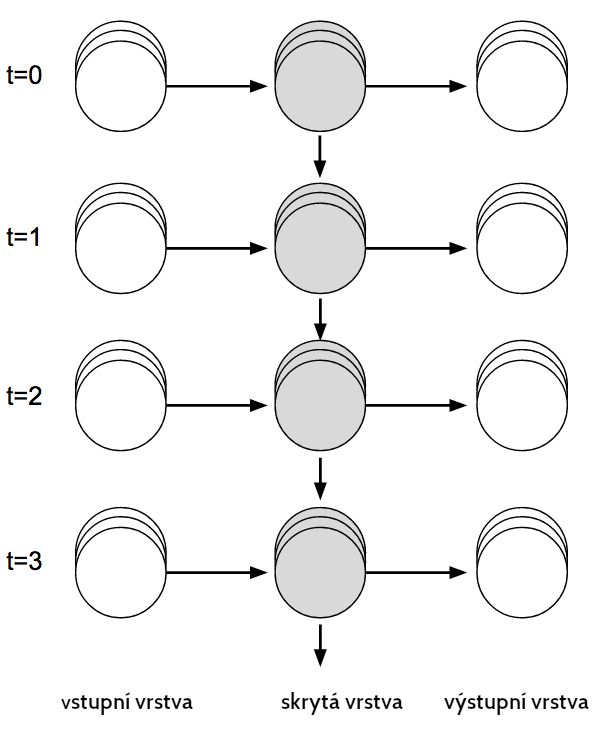
\includegraphics[scale=1]{rc/rnn1h.png}
\caption{
    Schéma rekurentní neuronové sítě. Vertikálně je znázorněn průběh času a
    horizontálně jednotlivé vrstvy sítě.
}
\label{fig:rnn}
\end{figure}

\begin{equation}
f_t = o_t tanh(c_t)
\end{equation}
kde
\begin{equation}
o_t = \sigma(W_{xo}x_t + W_{ho}h_{t-1} + W_{co}c_t + b_o),
\end{equation}
\begin{equation}
c_t = g_{t}c_{t-1} + i_t tanh(W_{xc}x_t + W_{hc}h_{t-1} + b_c),
\end{equation}
\begin{equation}
g_t = \sigma(W_{xg}x_t + W_{hg}h_{t-1} + W_{cg}c_{t-1} + b_g),
\end{equation}
\begin{equation}
i_t = \sigma(W_{xi}x_t + W_{hi}h_{t-1} + W_{ci}c_{t-1} + b_i),
\end{equation}
$\sigma$ je logistický sigmoid, $i$ je vstupní brána LSTM, $g$ je brána zapomnění
\textit{forget gate}, $o$ je výstupní brána, $c$ jsou aktivační vektory buňky
\textit{cell activation vectors}. $i$, $g$, $o$ i $c$ mají shodnou délku se
skrytým vektorem $h$. Na obrázku~\ref{fig:lstm} je vyobrazena buňka LSTM.

\begin{figure}[htpb]
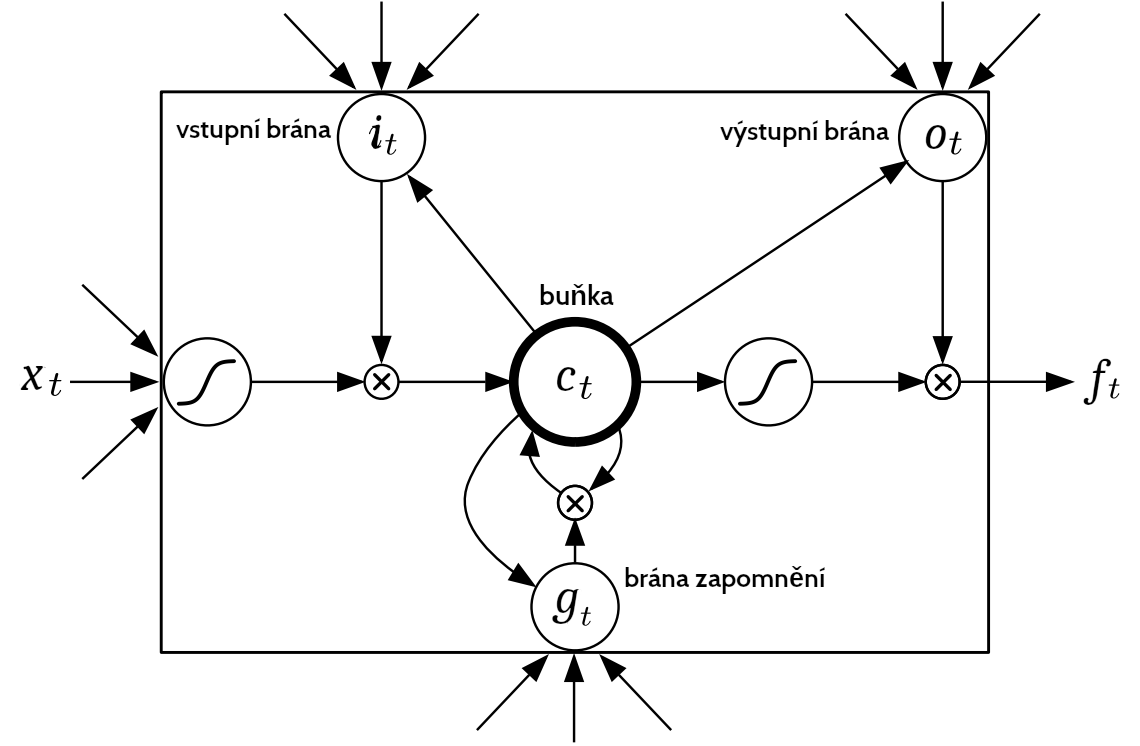
\includegraphics[scale=0.7]{rc/lstm.png}
\caption{
    Schéma buňky LSTM.
}
\label{fig:lstm}
\end{figure}

Síť je rekurentní v~obou směrech, neboť tomu nic nebrání, když vstupem jsou celé
věty. Prezentovaný systém proto využívá obousměrné LSTM, viz
obrázek~\ref{fig:birnn}. Ta definuje dopřednou skrytou vrstvu $\overrightarrow{h}$ jako
\begin{equation}
\overrightarrow{h}_t = f(W_{x\overrightarrow{h}}x_t + W_{\overrightarrow{h}\overrightarrow{h}}\overrightarrow{h}_{t-1} + b_{\overrightarrow{h}}),
\end{equation}
zpětnou skrytou vrstvu $\overleftarrow{h}$ jako
\begin{equation}
\overleftarrow{h}_t = f(W_{x\overleftarrow{h}}x_t + W_{\overleftarrow{h}\overleftarrow{h}}\overleftarrow{h}_{t-1} + b_{\overleftarrow{h}})
\end{equation}
a výstupy jako
\begin{equation}
y_t = W_{\overrightarrow{h}y}\overrightarrow{h}_t + W_{\overleftarrow{h}y}\overleftarrow{h}_t + b_o.
\end{equation}

\begin{figure}[htpb]
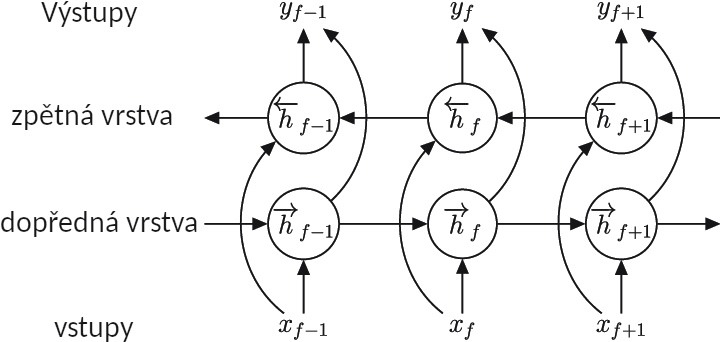
\includegraphics[scale=0.5]{rc/Bidirectional-recurrent-neural-network-50.png}
\caption{
    Schéma obousměrné rekurentní neuronové sítě
}
\label{fig:birnn}
\end{figure}

Použitá neuronová síť používá více skrytých vrstev, aby se umožnilo hluboké
trénování, takže pro N vrstev ($n = 1 .. N$) je vzorce třeba rozšířit:
\begin{equation}
h_t^n = f(W_{h^{n-1}h^n}h_t^{n-1} + W_{h^{n}h^{n}}h_{t-1}^n + b_h^n),
\end{equation}
kde $h^0 = x$.
\begin{equation}
y_t = W_{h^{N}y}h_t^N + b_o.
\end{equation}

Chybová funkce CTC je upravena tak, aby upřednostňovala kandidáty s~nízkou WER a
implementována pomocí metody Monte Carlo. Dekóduje se standardně pomocí
paprskového prohledávání \textit{(beam search)}. Systém natrénovaný na
jedenaosmdesátihodinové sadě z~Wall Street Journalu sice s~8,2\% WER nepřekonal
baseline implementovaný pomocí DNN-HMM se~7,8\%, ale to při tak malé trénovací
sadě není žádné překvapení, a i tak ukázal životaschopnost metody.

\subsection{Deep Speech}
\label{ssec:deepspeechpaper}

Na výše popsaný článek navázali ve výzkumném centru Baidu a navrhli systém
pojmenovaný DeepSpeech\cite{hannun2014deep}, který využívá tentýž přístup
s~důrazem na praktickou použitelnost a optimalizaci pro trénink na velkých
množstvích dat. Na rozdíl od Gravese 2014 používají jen jednu obousměrnou
rekurentní vrstvu a další čtyři skryté dopředné. Jako aktivační funkci ve
skrytých vrstvách používají místo sigmoidu shora omezené ReLu a na výstupu
standardní softmax. U dopředných vrstev se aplikuje dropout. Rekurentní vrstva
není LSTM z~důvodu optimalizace rychlosti. Obrázek~\ref{fig:deepspeech-arch}
znázorňuje architekturu sítě.

\begin{figure}[htpb]
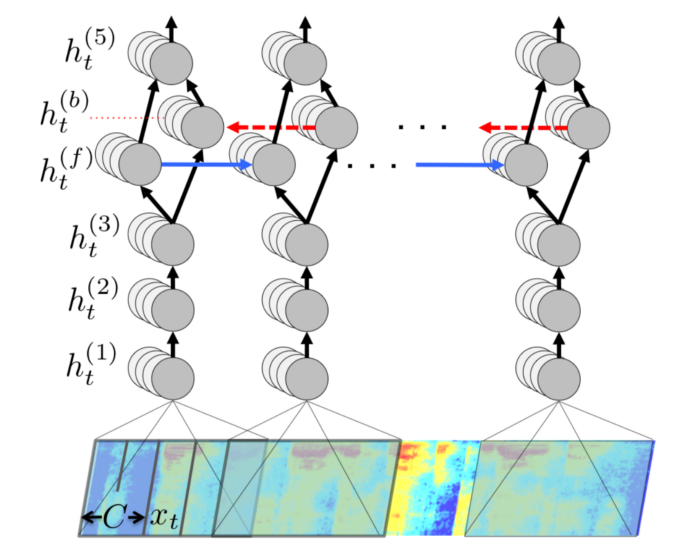
\includegraphics[scale=0.58]{rc/deepspeech-arch.png}
\caption{
    Architektura systému DeepSpeech.
}
\label{fig:deepspeech-arch}
\end{figure}

\section{Přepis Makoňova korpusu pomocí GMM-HMM}

%Až do druhé dekády druhého milénia byly nejlepší dostupnou technologií pro
%rozpoznávání řeči skryté markovovské modely s~gaußovskými směsmi (GMM-HMM).
%Architektura takového systému vypadá následovně:

%\begin{enumerate}
%\item{Diskrétní jednotkou vstupních dat je úsek přibližně o délce jedné věty.}
%\item{Vstupní datum\footnote{Datum ve smyslu jednotného čísla od slova data,
%z~latinského participia slova \textit{dare}, dát.} je zakódováno do posloupnosti
%reálněčíselných vektorů, z~nichž každý odpovídá setině sekundy signálu.}
%\item{}
%\end{enumerate}

%Pro získání počátečního přepisu bylo nutné sestavit
%systém pro automatický přepis, z~historických důvodů častěji označovaný jako
%rozpoznávání řeči. Rozpoznávání češtiny se věnovali mnozí přede mnou,
%například Ircing et al. (2001)\cite{ircing2001large}, Psutka et al.
%(2005)\cite{psutka2005automatic}, či Byrne et al. (1999)\cite{byrne1999large}.
%V následujících odstavcích popíšu tvorbu rozpoznávače řeči pro korpus Karla
%Makoně.

Zjednodušený řetězec vedoucí od~zvukových dat k~jejich přepisu v~našem případě
vypadá takto:\begin{enumerate}
\item{sběr trénovacích dat,}
\item{stavba akustického modelu,}
\item{stavba jazykového modelu,}
\item{automatické rozpoznávání.}
\end{enumerate}


V~průběhu práce jsem sestavil dva zcela odlišné akustické modely: Jeden založený
na skrytých markovovských modelech a jeden založený na neuronových sítích.
Hlavním důvodem bylo to, že když jsem začínal, nebyly ještě hluboké neuronové
sítě tak rozšířené. Jsou ale i dvě další výhody, které použití markovovských
modelů opodstatňují: 1) Nepotřebují tolik trénovacích dat, takže se více hodí do
začátku, kde je přepsaná množina malá,\footnote{První trénovací sadu jsem pořídil svépomocí přepisem asi 15 minut nahrávky
\texttt{85-05A}.} a 2) umožňují získat přesné zarovnání
slov a hlásek na časové pozice ve zvukovém záznamu. Dosud neznám žádný nástroj,
který by toto poskytoval bez použití HMM.

Nejdříve popíšu výstavbu markovovského modelu a poté
v~sekci~\ref{sec:deepspeech} se budu věnovat modelu založenému na neuronových
sítích.

%\section{Přepis Makoňova korpusu pomocí HMM}

%V~průběhu jedenácti let této disertační práce vznikly dva systémy automatického
%přepisu mluveného korpusu Karla Makoně. První z~nich, založný na skrytých
%markovovských modelech, popíšu v~této sekci.

Stěžejními nástroji pro tvorbu systému jsou 1) HTK pro akustický model, 2) KenLM
pro jazykový model a 3) Julius pro dekódování.

\subsection{Modelované hlásky}
\label{ssec:ac:fonetika}

Modeluji základní hlásky českého jazyka\cite{palkova1992fonetika}
reprezentované pomocí systému symbolů PACal\cite{nouza1997phonetic}. Kromě základních hlásek
používám dvojhlásky, ticho a krátkou pauzu. Ráz (glotální plozivu) nevyznačuji,
jakož ani neřečové události. Důvodem toho je, že vyznačování těchto jevů nelze
očekávat od anotátorů, se kterými tato práce počítá.
V~tabulce~\ref{tab:phones} jsou použité hlásky uvedeny.

\begin{table}[htpb]
%\fontspec{DoulosSIL}
\begin{center}
\begin{tabular}{|l|l|l||l|l|l|}
\hline
IPA                        & PACal & grafém & IPA & PACal & grafém \\
\hline
\textipa{a}                & a   & a      & \textipa{M}           & mg  & tra\underline{m}vaj \\
\textipa{a:}               & aa  & á      & \textipa{n}           & n   & \underline{n}e \\
\textipa{\t*{aU}}          & aw  & au     & \textipa{N}           & ng  & ta\underline{n}k \\
\textipa{b}                & b   & b      & \textipa{\textltailn} & nj  & \v{n} \\
\textipa{\t{ts}}           & c   & c      & \textipa{o}           & o   & o \\
\textipa{\t{tS}}           & ch  & č      & \textipa{o:}          & oo  & ó \\
\textipa{d}                & d   & d      & \textipa{\t*{oU}}     & ow  & ou \\
\textipa{\textbardotlessj} & dj  & \v{d}  & \textipa{p}           & p   & p \\
\textipa{\t{dz}}           & dz  & dz     & \textipa{r}           & r   & r \\
\textipa{\t{dZ}}           & dzh & dž     & \textipa{\|'{\r*{r}}} & rsh & t\underline{\v{r}}i \\
\textipa{E}                & e   & e      & \textipa{\|'r}        & rzh & \underline{\v{r}}íz \\
\textipa{E:}               & ee  & é      & \textipa{s}           & s   & s \\
\textipa{\t*{eU}}          & ew  & eu     & \textipa{S}           & sh  & š \\
\textipa{f}                & f   & f      & \textipa{t}           & t   & t \\
\textipa{g}                & g   & g      & \textipa{c}           & tj  & \v{t} \\
\textipa{H}                & h   & h      & \textipa{U}           & u   & u \\
\textipa{I}                & i   & i      & \textipa{u:}          & uu  & ú, \r{u} \\
\textipa{i:}               & ii  & í      & \textipa{v}           & v   & v \\
\textipa{j}                & j   & j      & \textipa{x}           & x   & ch \\
\textipa{k}                & k   & k      & \textipa{z}           & z   & z \\
\textipa{l}                & l   & l      & \textipa{Z}           & zh  & ž \\
\textipa{m}                & m   & \underline{m}ák
                                          &        & sil & \\
                           &     &        &        & sp  & \\
\hline
\end{tabular}
\caption{Použité hlásky: IPA, PACal a nejčastější odpovídající
grafém.}\label{tab:phones}
\end{center}
\end{table}
%\normalfont

V~závislosti na~množství trénovacích dat jsem nahrazoval některé hlásky
častějšími podobnými. V~tabulce~\ref{tab:phonesed} jsou záměny vyčísleny.
\begin{table}[htpb]
%\fontspec{DoulosSIL}
\begin{center}
\begin{tabular}{|r|l|l||l|l|}
\hline
&
\multicolumn{2}{|c||}{před záměnou} &
\multicolumn{2}{|c|}{po záměně} \\
\hline
& IPA & PACal & IPA & PACal \\
\hline
    & \textipa{M}       & mg & \textipa{m} & m \\
    & \textipa{\t*{aU}} & aw & \textipa{a U} & a u \\
    & \textipa{o:} & oo & \textipa{o} & o \\
\** & \textipa{\t{dz}}  & dz & \textipa{\t{ts}} & c \\
    & \textipa{\t{dz}}  & dzh & \textipa{\t{tS}} & ch \\
\** & \textipa{\t*{eU}} & ew & \textipa{E U} & e u \\
\hline
\end{tabular}
\caption{Použité záměny hlásek; hvězdičkou jsou vyznačeny záměny použité ještě
v~době psaní textu.}\label{tab:phonesed}
\end{center}
\end{table}
%\normalfont

\subsection{Tvorba akustického modelu}

\begin{enumerate}

\item{Vytvoření počátečních modelů.}

Všechny hlásky se inicializují jako
shodné. Každá hláska je reprezentována pěti stavy (vstupním, výstupním a třemi
vnitřními). Přechodové pravděpodobnosti se nastaví tak, aby byly možné jen
kýžené přechody, to jest ze~vstupního do~druhého a z~každého z~vnitřních stavů
do~sebe samého nebo do~následujícího. Pravděpodobnosti
se inicializují na 60\% pro setrvání a 40\% pro postup ve~druhém a
třetím stavu a 70\% pro setrvání a 30\% pro postup ze~čtvrtého do~výstupního.
Střed a variance jsou určeny identicky podle globálních hodnot.

V~této počáteční sadě je obsaženo ticho (\texttt{sil}), ale nikoliv krátká pauza
(\texttt{sp}). To se týká nejen parametru udávající množinu hlásek, ale také
trénovacího fonetického přepisu.
Pro kódování používám formát MFCC s~první a druhou derivací, základní frekvencí
a kepstrální normalizací (\texttt{MFCC\_0\_D\_A\_Z} v~notaci HTK).

Následují dvě iterace tréninku Baum-Welchovým algoritmem.

\item{Přidání modelu pro krátkou pauzu.}

Z~modelu pro ticho se odvodí model pro krátkou pauzu tak, že se povolí přechody
z~druhého do~čtvrtého stavu a zpět s~pravděpodobností 0,2 a ze vstupního do
koncového stavu s~pravděpodobností 0,3, aby byl model robustnější a mohl
modelovat pauzu mezi slovy, která je nezřídka nulová.

Stavy mezi modelem pro ticho a pro krátkou pauzu se sdílejí.
Trénuje se opět dvěma iteracemi BW-algoritmu, od teď již s~modelem pro krátkou
pauzu jak v~množině hlásek, tak ve fonetickém přepisu.

\item{Nucené zarovnání a odvržení zmetkových vzorků.}

Pomocí Viterbiho algoritmu\cite{forney1973viterbi} se provede tzv.
\textit{forced alignment}, tzn. nucené zarovnání na~úrovni hlásek. Jinými slovy
určí se přesný čas, kde začíná a končí která hláska. Při tom se určí hranice, pod
kterou když klesne \textit{likelihood} daného přepisu na~základě odpovídající
nahrávky, tato se z~trénovacích dat odstraní jako pravěpodobně vadná. Pro
zarovnání se použije Viterbiho algoritmus v~provedení programu HVite s~prahem
pro odmítnutí věty 150. Následují další dvě iterace BW-algoritmu.

\item{Přepočítání variance.}

Variance modelů byla určena podle původní trénovací sady. Nyní jsme z~ní
vyřadili některé vzorky, proto proběhne její přepočtení, opět následované dvěma
trénovacími iteracemi.

\item{Přechod k~trifónům}
\label{item:htktrain:triphones}

Z~nuceného zarovnání máme přepis obohacený o~konkrétní fonetické realizace. Z~té
se nyní snadno vytvoří přepis trifónový tak, že ke každé hlásce přidáme
jeho levý a pravý kontext, pokud nejsou na~začátku nebo na~konci věty.

Je-li hlásek 45, pak trifónů je až $45^3 = 91125$. Ne všechny se v~trénovacích
datech objeví. V~praxi jich mám kolem 14 tisíc. Pokud by každý trifón měl
vlastní separátní model, došlo by k~opačnému problému než v~případě monofónů,
totiž že by celkový model měl příliš mnoho parametrů. Přechodové matice mohou
všechny trifóny odvozené od jednoho monofónu sdílet. Avšak které trifóny
mají sdílet střed a varianci stavů a které mají mít vlastní, je třeba rozhodnout opatrněji.

Pro určení, které modely je vhodné sloučit, používám rozhodovací stromy.
Na~základě předem definovaných kritérií se u~každého emitujícího stavu každé
skupiny trifónů provede rozdělení na~dva shluky, což umožní zvýšení
\textit{log likelihood} dat. Vybere se kritérium, které log likelihood
zvýší nejvíce a postup se opakuje, dokud zvýšení neklesne pod~danou hranici.
Takto získané shluky se pak sloučí do jednoho logického trifónu.

Pro tvorbu rozhodovacích stromů je potřeba ručně vytvořit
otázky, na jejichž základě bude algoritmus dělit hlásky do shluků. K~tvorbě
otázek můžeme použít lingvisticky motivovanou kategorizaci v~naději, že aspoň
některé lingvistikou definované kategorie budou z~pohledu trénovacích dat tvořit
konzistentní shluky. Pro tvorbu otázek jsem vycházel z~předlohy pro
angličtinu, jak je uvedeno v~HTK Book, a z~kategorizace českých hlásek na Wikipedii
(\texttt{https://cs.wikipedia.org/wiki/Fonologie~češtiny}).
Otázky použité v~rozhodovacím stromě viz v~digitální příloze.
% TODO

\item{Přechod ke gaußovským směsem}

Posledním krokem ve~zvětšování komplexity modelu je přechod z~modelování stavů
prostými gaußovskými pravděpodobnostnímu distribucemi k jejich směsem
(angl. \textit{mixtures}). Spočívá v~tom, že se přesněji modelují variantní
realizace jednotlivých hlásek. Daná hláska v~jednom stavu HMM pak není modelována jednou gaußovskou
distribucí, nýbrž složením několika. Každá má svůj střed, svoji varianci a svoji
váhu, jejichž celkový součet musí být roven jedné.

Štěpí se vnitřní stavové modely jednotlivých hlásek. Optimální počet
složek směsi je tedy potřeba zjistit pro trojnásobek počtu použitých trifónů. To
jsou řádově tisíce až desítky tisíc. V~okamžiku psaní tohoto textu používám 8444
reálných trifónů; 13746, počítám-li i ty logické. To znamená přes dvacet pět
tisíc distribucí, u~nichž je potřeba určit optimální počet složek.

Aby byl úkol aspoň aproximací dosažitelný, je třeba hledat efektivněji než
prohledáváním celého prostoru hrubou silou. První pomocí zde je, že modely jsou
na sobě více méně nezávislé: Nalezneme-li optimální počet složek pro jeden
z~nich, nemělo by to ovlivnit optimální počet složek u~jiného.

Rozštěpení v~jedné směsi proběhne tak, že se složka s~největší vahou
rozštěpí na dvě totožné s~tím, že jedna dostane malinko větší váhu než druhá, aby se
při trénování mohly rozejít. To se provede u~všech vnitřích stavů všech
fyzických hlásek, t.j. u~všech markovovských modelů. Provedou se čtyři trénovací
iterace a úspěšnost se vyhodnotí na~sadě heldout.

Pokud u~některé složky klesne její váha pod~daný práh, vymaže se, čímž se
zamezí zbytečnému nárůstu parametrů, a není proto potřeba zkoušet štěpit
jednotlivé modely samostatně. Arci, štěpením modelů jednoho po druhém jsem nikdy nedosáhl lepšího
výsledku, než štěpením všech modelů najednou.

Závislost úspěšnosti na~počtu složek není monotónní, proto ve~štěpení pokračuji,
i když někdy úspěšnost klesne. Konkrétně zastavím štěpení, pokud úspěšnost
klesne o~více než 30\% oproti nejvyšší dosažené nebo pokud klesne více než
třikrát za~sebou, ne však když je složek méně než 16.

\end{enumerate}

%Pokud je hláska gaußiánem modelována dobře, rozdělení na dvě mixtury
%nijak nepomůže. Navíc pokud rozdělíme dostribuci příliš, dojde snadno
%k~přetrénování. Je proto potřeba nalézt optimální počet mixtur pro každý
%jednotlivý trifón.

\subsection{Dekódování}

Pro dekódování, čili samotný přepis na základě akustického a jazykového modelu,
používám nástroj Julius\cite{lee2001julius}. Julius pracuje na základě
dvouprůchodového algoritmu. Při prvním průchodu se využívá paprskového
prohledávání \textit{(beam search)} na slovníku s~vahami pro každé slovo zvlášť,
takže průchod je velmi rychlý a málo paměťově náročný. Datové struktury jsou
ponechány do druhého průchodu, který jde v~opačném směru a zapojuje n-gramový
jazykový model. V~tomto průchodu se hledá $k$ nejlepších kandidátů
v~\textit{trellis} (dosl. pergola; datová struktura) z~prvního průchodu.

\subsection{Jazykový model}
\label{sec:jazykovy-model}

Jazykový model obecně je odhad pravděpodobnostního rozdělení posloupností slov
v~přirozeném jazyce\cite{ponte1998language}. V~kontextu rozpoznávání řeči je tandemovým
partnerem akustického modelu\cite{jelinek1990self}. Teprve kombinace akustického
a jazykového modelu určí výsledné slovo, které se na dané pozici rozpozná jako
nejpravděpodobnější.

Výběr jazykového modelu je omezen nástrojem pro rozpoznávání. Lze zvolit pouze
takový model, který nástroj dokáže využít. Všechny nástroje, které jsem použil,
podporují N-gramové jazykové modely: HVite bigramový, Julius až trigramový a
DeepSpeech libovolného řádu.

Pro trénování jazykového modelu mám k dispozici čtyři druhy dat:
\begin{enumerate}
\item{Obecné české texty\footnote{Obecnými českými texty nemyslím texty v
{\em obecné češtině}, nýbrž obecné ve smyslu všech, které šlo opatřit.},}
\item{Makoňovy spisy,}
\item{manuální přepisy nahrávek,}
\item{automatické přepisy.}
\end{enumerate}

Každá z~těchto kategorií skýtá různé množství textu a různou věrnost
modelovanému materiálu. Nejvěrnější jsou samozřejmě manuální přepisy Makoňových
nahrávek, kterých je nejméně. V~okamžiku psaní tohoto textu je to 728 286
slov. Automatické přepisy, jejichž přínos pro jazykové modelování je nejasný,
představují 7 338 504 slov. Makoňovy spisy obsahují 3 328 720 slov. Obecné české
texty jsou nejdostupnější z~těchto komodit. Nejobsáhlejší dostupný korpus, který
jsem nalezl, je Mononews z WMT\cite{wmt19} obsahující 1 019 497 060 slov.

Inspirován výše zmiňovaným článkem od Psutky et al. 2003\cite{psutka2003large},
pokusil jsem se jejich přístup replikovat. Na základě předběžných pokusů jsem
zjistil, že nejlepší výsledek dává jazykový model natrénovaný z~Makoňových spisů
a manuálních přepisů, naopak přidání automatických přepisů nemá prakticky žádný
efekt. Výchozím bodem pokusu tedy byl reprezentativní korpus z~Makoňových textů
a korpus obecných českých textů. Cílem bylo vybrat z obecného korpusu ideální
podmnožinu vět vzhledem k~úspěšnosti rozpoznávání. Pro tyto účely jsem
natrénoval dva unigramové jazykové modely, jeden z~repezentativního (Makoňova)
korpusu: $M$ a druhý z~obecného (WMT): $W$.

První hledání proběhlo podle návodu ve zmiňovaném článku: Do trénovací sady
se vybraly ty věty $s$ z~obecného korpusu, které byly pravděpodobnější podle
modelu $M$ po aplikaci hledaného koeficientu $t$ než podle modelu $W$:
\begin{equation}
P(s|W) < t\cdot{}P(s|M)
\end{equation}
S~klesajícím $t$ a tím s~rostoucím počtem přidaných vět monotónně klesala
úspěšnost. Pohled na vybrané věty odhalil problém: byly to namnoze takové, které
byly velmi nepravděpodobné podle obecného modelu, takže špatně reprezentovaly
češtinu.

Druhé hledání proběhlo s~úpravou, že se použijí toliko věty, které nejsou
podle~reprezentativním modelu příliš nepravděpodobné. Průměrná \textit{log
likelihood} věty vážená počtem slov je v~reprezentativním modelu -3,51 a
standardní odchylka je 0,52. Práh pro inkluzi věty jsem tedy nastavil na -4.
Takto jsem došel ke zvýšení úspěšnosti o 2,7\%, z 0,112 na 0,109 WER.

U třetího hledání jsem zcela ignoroval pravděpodobnost věty podle obecného
modelu a rozřazoval pouze na základě pravděpodobnosti podle reprezentativního
modelu. Touto metodou jsem dosáhl zvýšení úspěšnosti o 8,0\% z~0,112 na 0,103
WER.

Vývoj úspěšnosti podle kritéria přidání vět z~obecného korpusu do jazykového
modelu shrnuje tabulka~\ref{tab:lm-plz-scores} a
obrázek~\ref{fig:lm-plz-scores}.
Výsledek považuji za zajímavý, neboť shledává jinou, dokonce jednodušší metodu
v~tomto případě účinnější než navrhovanou autory.

\begin{table}[htpb]
\begin{center}
\begin{tabular}{|l|r r r|r|}
\hline
kritérium & \multicolumn{3}{c|}{počet přidaných vět} & WER \\
                        &       \# &  \%W       & $\div{}M$ & \\
\hline
Ø                       &        0 &  0,000\% &  0,00 & 11,2\% \\
$l<0,65m$               &   715246 &  0,991\% &  2,09 & 11,5\% \\
$l<0,8m$                &  2629381 &  3,644\% &  7,70 & 11,6\% \\
$l<m$                   & 10263276 & 14,223\% & 30,05 & 11,7\% \\
$l<0,65m$ \& $m>10^{-4}$&   217359 &  0,301\% &  0,64 & 11,2\% \\
$l<0,8m$ \& $m>10^{-4}$ &  1466100 &  2,032\% &  4,29 & 11,0\% \\
$l<m$ \& $m>10^{-4}$    &  6587540 &  9,129\% & 19,29 & 10,9\% \\
$l<1,3m$ \& $m>10^{-4}$ & 14544308 & 20,156\% & 42,58 & 11,2\% \\
$m>10^{-2}$             &     2380 &  0,003\% &  0,01 & 11,1\% \\
$m>10^{-2,5}$           &    61654 &  0,085\% &  0,18 & 11,0\% \\
$m>10^{-2,8}$           &   308102 &  0,427\% &  0,90 & 10,6\% \\
$m>10^{-3}$             &   786947 &  1,091\% &  2,30 & 10,4\% \\
$m>10^{-3,2}$           &  1790919 &  2,482\% &  5,24 & \textbf{10,3\%} \\
$m>10^{-3,3}$           &  2598266 &  3,601\% &  7,61 & 10,3\% \\
$m>10^{-3,51}$          &  5246049 &  7,270\% & 15,36 & 10,6\% \\
$m>10^{-4,03}$          & 19282850 & 26,723\% & 56,45 & 11,2\% \\
\hline
\end{tabular}
\caption{Úspěšnost rozpoznávání s~použitím různých částí obecného korpusu.
Kritérium rozhoduje o zařazení věty do jazykového modelu. Proměnná $m$ je
pravděpodobnost věty podle unigramového modelu z~Makoňových přepisů a spisů,
vážená počtem slov. Proměnná $w$ je totéž podle modelu z~obecných českých textů.
Počet přidaných vět je uveden v~celkovém počtu, v~procentech celkové velikosti
obecného korpusu a v~násobcích velikosti reprezentativního korpusu.}\label{tab:lm-plz-scores}
\end{center}
\end{table}

\begin{figure}[htpb]
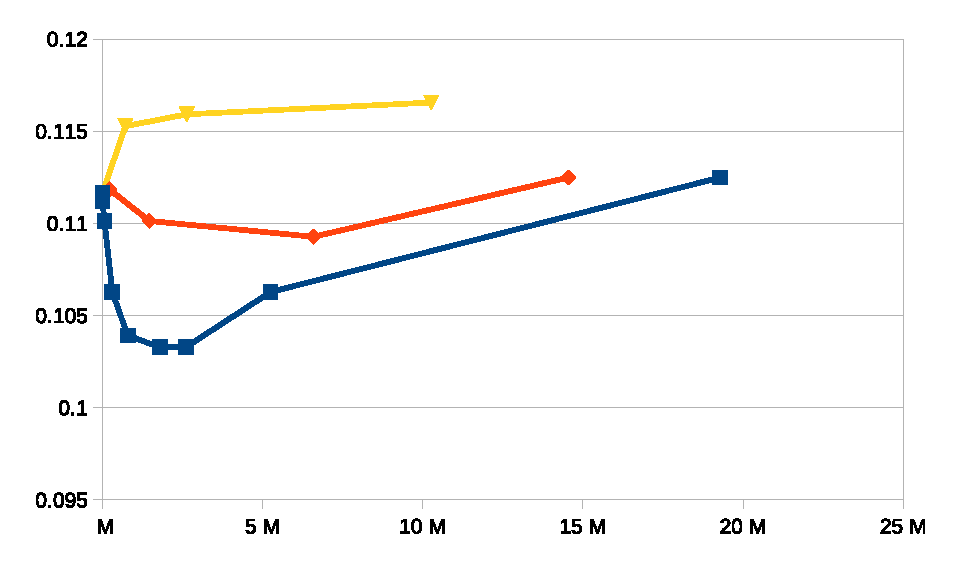
\includegraphics[scale=0.9]{rc/lm-plz-scores.eps}
\caption{
  Hledání optimální podmnožiny obecného korpusu pro jazykové modelování. Na ose
  X je počet přidaných vět, na ose Y WER. Žlutá čára s trojúhelníčky
  reprezentuje první pokus (řádky 2-4 v~tabulce~\ref{tab:lm-plz-scores});
  Červená čára s~čtverečky na hrotech druhý pokus (řádky 5-8); modrá čára
  s~čtverečky na stranách třetí pokus (řádky 9-16).
}
\label{fig:lm-plz-scores}
\end{figure}

Jazykový model stavím pomocí nástroje KenLM\cite{heafield2011kenlm}. Aplikuji
vyhlazování technikou Knesser-Ney\cite{chen1999empirical}, jak je v něm
zabudována.

Je třeba podotknout, že u manuálních přepisů dochází k~jednomu
nežádoucímu jevu. Přepisy se pořizují tak, aby byly maximálně věrné tomu, co je
vyřčeno. Proto se doslova... vlastně do hlásky přepisují i přebrepty a zadrhnutí.
Je otázkou, zda takové jevy chceme mít v~jazykovém modelu. Aniž bych se na ni
pokoušel poskytnout definitivní odpověď, můj přístup, jak se s~tímto vypořádat,
je, instruovat uživatele těmito pokyny: 1) Každé slovo, po kterém následuje přerušení toku
mluvy doplnit třemi tečkami,
2) pokud se mluvčí zadrhne uprostřed slova nebo vysloví něco, co není slovem,
připojit k~tomuto útvaru pomlčku\footnote{Standardní postup, se kterým jsem se
seznámil až později, je místo pomlčky použít symbol \texttt{+}.}. Například ve větě {\em ,,To je ta relativnost
dobrého a zlého, tak kdybychom... to je tam jinak postaveno.``} patří tři tečky
za slovo {\em kdybychom}. Ve větě {\em ,,To je první š- špatný pohled, chybný pohled na rodiče a na
předcházející generaci.``} patří pomlčka za vyslovené {\em š}, za kterým
teprve následuje vyslovené slovo {\em špatný}.

Při stavbě jazykového modelu toto značení umožní, aby se věta při setkání
s~takovým slovem ukončila nebo aby se takové slovo přeskočilo.

%\section{Segmentace}
%
%Zpravidla jeden zvukový soubor odpovídá jednomu přetočení magnetofonové pásky,
%obvyklá délka je tedy 45 až 120 minut. Takto dlouhé úseky nelze použít ani jako
%trénovací příklady ani jako cíl automatického rozpoznávání.
%
%Sofistikovanější segmentaci popisuji v~sekci~\ref{sec:segmenty}. Pro účely
%vývoje iniciálního systému automatického přepisu jsem však použil jednodušší
%metodu:
%
%Celá aplikace je pojata jako nástroj pro~zdokonalování automatického přepisu,
%takže vychází z~předpokladu, že nějaký přepis již existuje. Vycházeje z~téhož
%předpokladu při~segmentaci, realizoval jsem ji tak, že zvukový soubor se rozdělí
%na~úseky odpovídající jednotlivým větám v~přepisu, ne však delší než patnáct
%sekund. Pokud by věta byla delší, rozdělí se u nejbližšího slova
%před~patnáctisekundovou hranicí.
%
%V~případě, že pro daný záznam zatím žádný přepis neexistuje, rozdělí se naivně
%na~patnáctisekundové úseky.

\section{Rozdělení dat}
\label{sec:asr:rozdeleni-dat}

Pro natrénování modelu strojovým učením je potřeba trénovacích dat a pro
vyhodnocení jeho úspěšnosti dat testovacích, která ve~fázi trénování nesmí být
algoritmem spatřena. Při trénování samotném se pak mnohdy používá vyhrazených,
tzv.~\textit{heldout} dat\footnote{Často zaměňovaných s~vývojovou testovací sadou
označovanou běžně jako \textit{dev} / \textit{dtest}.} pro průběžné měření úspěšnosti. V~případě trénování
akustického modelu s~použitím HTK je tomu nejinak. Heldout data jsou používána
pro zjištění optimálního počtu složek v~gaußovských směsích modelů jednotlivých hlásek a testovací
data jsou používána pro závěrečné vyhodnocení.

Anotovaná data mi přibývala velice pozvolna. Začínal jsem s~několika minutami,
ovšem přírůstky byly časté. Nemohl jsem si tedy dovolit udělat od~začátku pevnou
testovací sadu, kterou bych používal po~celou dobu provádění experimentů. Místo
toho jsem s~každou novou dávkou anotovaných dat celou sadu rozdělil podle vět
v~poměru 18:1:1 do trénovací, heldout a testovací sady. Tak jsem měl neustále
vyvážený poměr jednotlivých datových sad. Zřejmou velkou nevýhodou bylo, že
nešlo spolehlivě porovnávat výsledky jednotlivých experimentů vzhledem
k~variabilní testovací sadě.

Až když jsem měl několik desítek hodin anotovaných dat, vyhradil jsem si fixní
testovací sadu. Běžně se testovací sada vybere jako náhodná podmnožina vzorků
z~trénovací sady tak, aby měla kýženou velikost. V~mém případě vzorků zvíci
hodinových nahrávek jsem sadu určil manuálně jako úsek druhé až jedenácté minuty
(tedy deset minut, vždy jednu minutu po~začátku) v~pěti nahrávkách,
\begin{enumerate}
\item{jedné kazety z~roku 1976,}
\item{jedné z~roku 1982,}
\item{jedné z~roku 1986,}
\item{jedné z~roku 1990 a}
\item{jednoho nedatovaného kotouče.}
\end{enumerate}

Sadu heldout nyní vybírám jako každou čtyřicátou větu. Z~každé dvacáté jsem
snížil na~polovic nejen abych neplýtval trénovacími daty, nýbrž také protože
vyhodnocování směsí zabírá při trénování zdaleka nejvíce času, a ten je přímo
úměrný velikosti sady heldout.

\section{Experiment s kepstrální normalizací}
\label{sec:mfcc-norm}

Kepstrální normalizace je standardní technikou pro kompenzaci různorodých
akustických podmínek v~rámci trénovacích a testovacích dat, viz Viikki a Laurila
(1998)\cite{viikki1998cepstral}. Princip této techniky spočívá v~tom, že se ode
všech melfrekvenčních kepstrálních koeficientů odečte jejich průměr z~akusticky
konzistentního úseku. Já toto poněkud hrubiánsky činím na celých nahrávkách,
které nejsou vždy akusticky konzistentní. Často však ano a nalezení akusticky
podobných množin je jedním z~mých plánů pro budoucí práci.\footnote{Tato úloha
je již vyřešena a popsána v~sekci~\ref{sec:akustika:metrika} a následující.}

Nabízí se však otázka, zda má smysl odečítat průměr z~celé nahrávky, nebo by to
mělo být jen z~řečových událostí, tedy s~vynechaným tichem (šumem, hluky atd.)
Tato idea, přišedší ke mně od dr. Davida Klusáčka, mne zaujala natolik, že jsem se
ji pokusil ověřit. Vytvořil jsem proto metadata s~časovými pozicemi všech
izolovaných řečových událostí na základě zarovnaného automatického přepisu a sadu skriptů
pro manipulaci se soubory MFCC.

Ke každému souboru MFCC jsem vytvořil kopii, ze které
jsem odstranil všechny výskyty hlásek \texttt{sil} a \texttt{sp}. Průměry kepstrálních
koeficientů jsem pak spočetl na těchto kopiích a odečetl je od hodnot
v~originálech. Trénování i testování jsem pak prováděl na takto upravených
souborech místo standardní normalizace, jak ji poskytuje systém HTK.

S~použitím takto normalizovaných nahrávek se chybovost na slovech snížila ze
46,4\% na 45,9\%.  Aparát pro dekódování
a manipulaci souborů MFCC považuji za vítaný vedlejší produkt.

\section{Aktivní učení}

Aktivní učení spočívá ve vhodném výběru trénovacích dat, viz např. Cohn
(1996)\cite{cohn1996active}. V~mém případě trénovací sada postupně roste a nabízí
se tedy využít techniky aktivního učení tak, aby se získávala co nejvhodnější
trénovací data.

Podnikl jsem experiment, ve kterém jsem ve webovém rozhraní ke sběru trénovacích
dat (viz kapitolu~\ref{kap:webove-rozhrani}) slova s~nízkou {\em confidence
measure (c.m.)} (pod 0,3) podtrhl červenou přerušovanou čarou, jejíž sytost spojitě rostla
s~klesající c.m. Instruoval jsem pak uživatele aplikace, aby přednostně
přepisovali věty, které jsou opticky co nejčervenější. Bohužel přirozené puzení
uživatelů přepisovat nahrávku kompletně a lineárně od začátku způsobilo, že
přepisů, kde se tato instrukce dodržuje, je zcela mizivé množství.

Druhý experiment spočíval v~tom, že webová aplikace sama vybírala věty pro
přepis na základě toho, kolik obsahovala slov s~nízkou c.m. Uživatelé pak byli
instruováni, aby nahrávku jen poslouchali, a opravu vložili, až když se
přehrávání samo přeruší. Tento pokus skončil neúspěchem, neboť
změna v~chování aplikace byla pro uživatele natolik nepříjemná, že jsem je
raději navrátil do původního.

\section{Rozšíření trénovací množiny}
\label{sec:confident}

Skóre confidence measure se dá využít ještě jiným způsobem: lze vybrat
úseky v~korpusu kromě testovací sady\footnote{K zamyšlení: je zde opravdu nutné
vynechat testovací data?}, kde automatický přepis uvádí vysokou míru
c.m. a přidat tyto úseky do trénovací množiny. Tento experiment jsem provedl
tak, že minimální délku úseku jsem stanovil na 1 sekundu, minimální počet
obsažených hlásek na 10 a minimální c.m. na 0,6. Práh 0,6 jsem určil namátkovou
kontrolou, která poukazovala na zanedbatelnou chybovost takových úseků. Celkem
tento výběr poskytl 99 hodin audia, tedy 10\% celého korpusu.
Chybovost rozpoznávání se zvýšila ze 46,4\% na 49,4\% a doba trénování
se zvýšila také.

\section{ASR na parlamentním korpusu}
\label{sec:csasr:results}

Po rozšíření hlubokých neuronových sítí došlo k~pokusu o přepis pomocí systému
na nich založeného. 
Hluboké neuronové sítě našly využití
snad ve všech oblastech strojového učení, viz např. LeCun
(2015)\cite{lecun2015deep}, Hinton (2012)\cite{hinton2012deep}. Toto neminulo ani
rozpoznávání řeči, konceptuelně již dávno před tím, viz Morgan
(1995)\cite{morgan1995neural}.
Nezisková organizace Mozilla vydala vlastní svobodný nástroj pro rozpoznávání
řeči DeepSpeech\cite{hannun2014deep} založený na
TensorFlow\cite{abadi2016tensorflow}, který implementuje práci popsanou
v~podsekci~\ref{ssec:deepspeechpaper}.
Na rozdíl od článku\cite{hannun2014deep} však implementuje rekurentní vrstvu
pomocí LSTM upřednostňuje přesnost modelu před komputační efektivitou.

Dříve než popíšu použití neuronových sítí pro přepis Makoňova korpusu,  pojednám
o použití datové sady představené v~kapitole~\ref{kap:svolocz} pro rozpoznávání
řeči.
Zmíněnou datovou sadu jsem použil pro natrénování rozpoznávače řeči pomocí
systému DeepSpeech. Sadu jsem
rozdělil na trénovací (train), ladicí (dev) a testovací (test)\footnote{Toto
označení je v~souladu s~konvencí pro systém DeepSpeech, ale ve skutečnosti jde
po řadě o množiny train, heldout a dtest, jak zmiňuji v~sekci~\ref{sec:asr:rozdeleni-dat}.} v~poměru 18:1:1.
Hyperparametry jsem nastavil následovně: learning rate 0,0001, dropout rate 0,2,
zbytek ponechán defaultně. Ke konvergenci došlo po 12 epochách.
S~použitím pentagramového jazykového modelu natrénovaného na
stenografických přepisech byla výsledná WER 8,40\% před expanzí číslic a 7,89\% po expanzi.

Ze zdrojů zmíněných v~úvodu kapitoly~\ref{kap:svolocz} se bez větší námahy se ziskem v~řádu
aspoň desítek hodin daly použít 1) Otázky Václava Moravce a 2) Vystadial. Krom
toho jsem použil veřejně nepřístupné zdroje 3) CUCFN -- Korpus Finančních zpráv
Univerzity Karlovy, 4) Korpus reprezentativní mluvené češtiny
Oral2013\cite{oral2013} a 5) amatérsky namluvenou Bibli, která je dostupná na adrese
\texttt{poslouchamebibli.cz}, a u které není žádná explicitní licence.

Na všech sadách včetně manuálních přepisů nahrávek Karla Makoně jsem natrénoval
model s~použitím téhož systému Mozilla DeepSpeech, týchž hyperparametrů a téhož
obecného jazykového modelu. Ten jsem natrénoval na datech z~WMT
2019\cite{wmt19}.

Nakonec jsem natrénoval akustický model na všech trénovacích
sadách sloučených do jedné.
Tabulka~\ref{tab:csasr:results} shrnuje word error rate systémů trénovaných na
jednotlivých částech testovaných jednak na testovací sadě z~téhož zdroje a
jednak na agregované testovací sadě sloučené ze všech dílčích.
Z~důvodu použití obecného jazykového modelu je u parlamentního korpusu vyšší chybovost než
výše zmiňovaných 8,40\% a u Makoňova korpusu taktéž vyšší chybovost než 19\%
uvedených v~sekci~\ref{sec:deepspeech}.

\begin{table}[htpb]
\begin{center}
\begin{tabular}{|l||r|r|}
\hline
zdroj     & WER na sobě & WER na všech \\
\hline
bible     & 9,20\%  & 94,7\% \\
cucfn     & 31,6\%  & 72,8\% \\
makoň     & 30,4\%  & 77,3\% \\
oral2013  & 78,4\%  & 60,7\% \\
ovm       & 21,6\%  & 72,9\% \\
parlament s~číslicemi & 8,74\%  & 39,7\% \\
parlament ve slovech  & 7,89\%  & 36,0\% \\
vystadial & 51,0\%  & 74,0\% \\
\hline
vše s~číslicemi   & 28,4\%  & 28,4\% \\
vše ve slovech    & 26,0\%  & 26,0\% \\
\hline
\end{tabular}
\caption{Word error rate rozpoznávání řeči na jednotlivých korpusech a na jejich
konkatenaci.}\label{tab:csasr:results}
\end{center}
\end{table}

%           cstest      selftest
% ovm       0.728954    0.216131
% bible     0.947226    0.091958
% cucfgn    0.728446    0.316287
% vystadial 0.739838    0.509930
% svolocz   0.397490    0.083978
% makon     0.773216    0.191772
% oral2013  0.607015    0.783525
% all       0.283574    0.283574
%
% cucfgnOF  0.683059    0.141142
% all\o                 0.130555

\section{Přepis Makoňova korpusu pomocí neuronových sítí}
\label{sec:deepspeech}

Pro přepis Makoňova korpusu jsem natrénoval dva akustické modely pomocí DeepSpeech:
1) čistě na manuálních přepisech
Makoňových nahrávek (v~té době 100 hodin), 2) na agregované sadě popsané
v~sekci~\ref{sec:csasr:results}. Používal jsem parametr \textit{automatic mixed
precision} pro rychlejší trénink, \textit{batch size} 50, \textit{dropout} 0,2 a
\textit{learning rate} $1^{-4}$.

Model natrénovaný jen na Makoňových nahrávkách zkonvergoval po osmi epochách a
dosáhl word error rate 19,2\% na testovací sadě. Druhý model jsem vytvořil tak,
že jsem nejprve trénoval na agregované trénovací sadě s~použitím Makoňovy
sady heldout pro validaci. Tato část zkonvergovala po 15 epochách a dosáhla WER
16,6\%. Následně jsem pokračoval v~tréninku na Makoňových nahrávkách. Tato část
zkonvergovala po dvou epochách a konečné skóre bylo 13,0\% WER.

Dokud jsem ale trénoval s~číslicemi, viz sekci~\ref{sec:svolocz:cislovky},
dosáhl tento model výrazně nižší úspěšnosti s~téměř dvojnásobnou chybovostí
27,3\% resp. 23,5\% WER.
Na testovací sadě měl tedy vyšší úspěšnost model trénovaný jen na 100h Makoňových
nahrávek se standardní abecedou, předče model trénovaný na 1500 hodinách na
abecedě rozšířené o číslice.


Nejmarkantnější zlepšení přináší robustní model na velice poškozených nahrávkách, které jsem
v~době výběru testovací sady ještě neměl k~dispozici, any byly digitalizovány
mnohem později. Jedná se hlavně o nahrávky pořizované při nízké rychlosti
převíjení pásky, zmiňované jednak v~sekci~\ref{sec:akustika:kompenzace} a jednak
v~sekcích~\ref{sec:data:rec} a \ref{sec:data:digitisation}.

Na minutovém úseku jedné z~nejpoškozenějších nahrávek, který jsem
přepsal, má první model WER 94,1\%, zatímco robustní model má WER
75,8\%. Porovnání na větším, asi pětiminutovém úseku je uvedeno
v~sekci~\ref{sec:akustika:vyhodnoceni}.

Bohužel vinou přímého mapování z~parametrizovaného audia na grafémy přicházíme o
možnost zarovnání na úrovni hlásek, takže je nutno výstup nechat zarovnat
v~další iteraci, aby se umožnilo synchronní přehrávání ve webovém rozhraní.

\section{Úspěšnost}
\label{sec:evaluace}

Poslední naměřená word error rate markovovského akustického modelu s~výše zmíněným
jazykovým modelem je 46,3\%. Nejnižší dosažená WER s~pentagramovým jazykovým
modelem popsaným v~sekci~\ref{sec:jazykovy-model} je \textbf{10,3\%}.

Jelikož jsem zpočátku práce neměl žádná přepsaná data, určil jsem fixní testovací sadu
až v~průběhu projektu. Chybí v~ní přepisy těch
nejméně srozumitelných nahrávek, které byly digitalizovány až po provedení
většiny experimentů, a navíc k~nim pořizovat ruční přepisy je velice nesnadné.

Tabulka~\ref{tab:asr-scores} uvádí nejdůležitější milníky ve word error rate
s~použitím trigramového jazykového modelu natrénovaného na Makoňových spisech a
manuálních přepisech. Je
s~podivem, že model dotrénovaný na Makoňových nahrávkách má na obecné testovací
množině větší úspěšnost (v~tabulce tučně) než výchozí model trénovaný na všech datech
(viz tabulku~\ref{tab:csasr:results}). Dalo by se čekat, že
když se po konvergenci na obecné trénovací množině aplikují ještě
další trénovací epochy na jiných specifických datech, měla by úspěšnost stoupnout na
oněch specifických datech a poklesnout na datech obecných. Příčinu tohoto jevu
jsem dosud neměl příležitost prozkoumat.

\begin{table}[htpb]
\begin{center}
\begin{tabular}{|l|l|l|l|}
\hline
model & GMM & \makecell{ DNN trénovaný\\ na Makoňovi } & \makecell{ DNN trénovaný\\ na různých sadách } \\
\hline
\makecell{standardní testovací\\ množina (50min)} & 46,3\% & 19,2\% & \textbf{13,0\%} \\ \hline
\makecell{5 minut\\ přebuzených záznamů} & & 45,0\% & 34,8\% \\ \hline
\makecell{5 minut\\ záznamů pořízených\\ nízkou rychlostí } & & 68,5\% & 42,1\% \\ \hline
\makecell{1 minuta obzvláště\\ nesrozumitelného záznamu } & & 94,1\% & 75,9\% \\ \hline
\makecell{agregovaná testovací\\ sada z~různých dat} & & 77,3\% & \textbf{22,2\%} \\ \hline %25,3 s číslicema
\end{tabular}
\caption{Chybovosti tří důležitých modelů na různých testovacích sadách s~trigramovým
jazykový modelem trénovaným na Makoňových přepisech a spisech.}\label{tab:asr-scores}
\end{center}
\end{table}

Je úspěšnost nízká nebo vysoká? V~roce 2016 publikovali Mizera et
al.\cite{mizera2016kaldi} sadu receptů na rozpoznávání řeči pro češtinu.
Uvádějí jako state of the art techniky GMM-HMM a DNN-HMM a word error rate pro
jednotlivé recepty mezi 8,49 a 48,47 podle povahy dat. Úspěšnost na korpusu
Karla Makoně v~tomto porovnání je velmi dobrá, obzvláště s~přihlédnutím
k~velké akustické variabilitě materiálu.

Na závěr kapitoly uvádím na obrázku~\ref{fig:asrhist} vývoj úspěšnosti
automatického přepisu mluveného korpusu Karla Makoně od prvních experimentů po
současnost.
\begin{itemize}
\item{
  První sloupec odpovídá iniciálnímu přepisu modelem založeným na
systému HTK natrénovaným na necelých čtyřech hodinách vlastních přepisů
pořízených pomocí prototypu webové aplikace.
}
\item{
  Druhý, čtvrtý, pátý a devátý sloupec odpovídají milníkům v~nárůstcích
  přepsaného materiálu použitého jako trénovací data.
}
\item{
  Třetí sloupec značí odstranění triviální chyby použití nesprávné
  vzorkovací frekvence, tedy přechod ze 44100~Hz na 16~kHz.
}
\item{
  Šestý sloupec koresponduje s~experimentem kepstrální normalizace popsaným
  v~sekci~{sec:mfcc-norm}.
}
\item{
  Sedmý sloupec odpovídá pokusu o přidání řídkých hlásek:
  \textipa{\t*{aU}}, \textipa{M}, \textipa{o:} a \textipa{\t{dZ}}.
}
\item{
  Osmý sloupec odpovídá pokusu štěpit složky ve směsích modelů jednotlivých
  hlásek, nikoliv všechny najednou.
}
\item{
  Desátý sloupec odpovídá pokusu o rozšíření trénovací sady o automaticky
  přepsané pasáže mluveného korpusu Karla Makoně s~velkou mírou jistoty
  predikce.
}
\item{
  Jedenáctý sloupec odpovídá prvnímu modelu na bázi DeepSpeech, kde k~trénování
  bylo použito týchž sto hodin Makoňových nahrávek jako u předcházejícího modelu
  na bázi HTK v~devátém sloupci.
}
\item{
  Dvanáctý sloupec odpovídá modelu trénovanému pomocí DeepSpeech na
  sedmnáctisethodinové trénovací sadě z~různých zdrojů.
}
\end{itemize}

\begin{figure}[htpb]
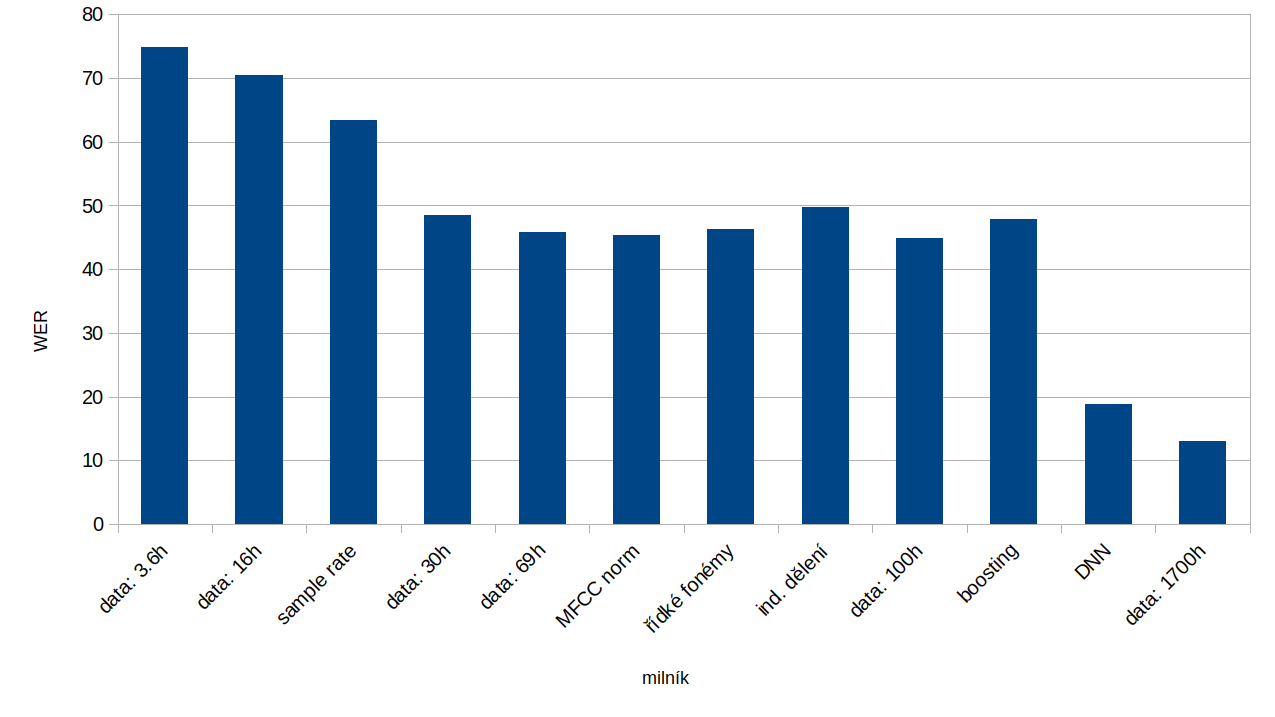
\includegraphics[scale=1]{rc/asrhist.png}
\caption{
    Vývoj úspěšnosti přepisu.
}
\label{fig:asrhist}
\end{figure}
